\documentclass[letterpaper, 12pt]{article}

% imports
\usepackage{amsmath}
\usepackage{amssymb}
\usepackage{anyfontsize}
\usepackage{array}
\usepackage[english]{babel}
\usepackage{braket}
\usepackage{enumitem}
\usepackage[margin=1in]{geometry}
\usepackage{graphicx}
\usepackage{hyperref}
\usepackage[utf8]{inputenc}
\usepackage{setspace}
\usepackage{tikz}
\usepackage{titlesec}
\usepackage{xcolor}

% configure imports
\definecolor{linkcolour}{rgb}{0, 0.2, 0.6}
\hypersetup{colorlinks, breaklinks, urlcolor=linkcolour, linkcolor=linkcolour}


\begin{document}

\begin{center}
  {\huge Schuster Lab - GRAPE 2.0 Proposal} \\[0.5em]
  {\large Thomas Propson $\vert$ \href{mailto:tcpropson@uchicago.edu}
    {tcpropson@uchicago.edu} \\[0.5em] \today}
\end{center}

\section{Motivation}
%% "Don't call it a comeback; I've been here for years" LL Cool J.

There are tasks we would like to perform that GRAPE 1.0 \cite{leung2017speedup} does not support. Additionally, there are performance improvements that can be made. We list them here:
\begin{enumerate}
\item GRAPE 1.0 uses Tensorflow to perform automatic differentiation. Tensorflow is a heavy-handed choice for the task at hand. It still does not support automatic differentiation with complex inputs. Therefore, it requires us to perform complex to real, and vice-a-versa, transformations in our code. It stores intermediate propagators and state vectors in its computation graph, using memory uneccessarily. Both storing the computation graph and waiting for a Tensorflow session to perform tensor operations incorporates unecessary boilerplate that can be shed.
  
\item GRAPE 1.0 does not support arbitrary relationships between control amplitudes and control operations. GRAPE 1.0 does not allow relationships between one control amplitude and more than one control hamiltonian (e.g. it does not allow $H = \epsilon(t)H_{control, 1} + \epsilon(t)^{*}H_{control, 2}$). Furthermore, GRAPE 1.0 restricts the relationship between control amplitudes and control hamiltonians to be linear (e.g. it does not allow $H = \epsilon(t)^{2}H_{control}$). Both of these examples occur in the Piccolo Hamiltonian:
\begin{align*}
  H &= \omega_{f}\ket{f}\bra{f} \\
  &+ \omega_{e}\ket{e}\bra{e}\\
  &+ \epsilon_{ge}e^{i\omega_{d}t}\ket{g}\bra{e} + \epsilon_{ge}^{*}e^{-i\omega_{d}t}\ket{e}\bra{g}\\
  &+ \epsilon_{ef}e^{i\omega_{d}t}\ket{e}\bra{f} + \epsilon_{ef}^{*}e^{-i\omega_{d}t}\ket{f}\bra{e}\\
  &+ \omega_{c}a^{\dagger}a\\
  &+ \chi_{e}\ket{e}\bra{e}a^{\dagger}a + \chi_{f}\ket{f}\bra{f}a^{\dagger}a\\
  &+ \epsilon_{sb}e^{i\omega_{d}t}\ket{f}\bra{g}a + \epsilon_{sb}^{*}e^{-i\omega_{d}t}\ket{g}\bra{f}a^{\dagger}\\
  &+ \epsilon_{sb}^{2}(\eta_{e}\ket{e}\bra{e} + \eta_{f}\ket{f}\bra{f})\\
\end{align*}
  Additionally, GRAPE 1.0 does not allow for time-dependent drift hamiltonians. For example, the qubit frequency in flux-tunable qubits is a function of flux through its junction, which is time-dependent.

\item In GRAPE 1.0, it is difficult to have complete control over the cost functions used in optimization and control their weights. For example, the fidelity cost function is always implicitly used but the user has no frame of reference to choose values for the regularization coefficients specified for other cost functions.
  
\item Better numerical approximation techniques can be used (e.g. matrix exponentiation, numerical integration, etc.).

\item There are opaque naming conventions and code formatting used in GRAPE 1.0. GRAPE 1.0 is hard to extend.
\end{enumerate}

\section{Automatic Differentiation}
We will use \href{https://github.com/HIPS/autograd}{Autograd} \cite{maclaurin2016modeling} for short operations in GRAPE 2.0. It supports gradients of functions that take complex inputs and return real outputs. This covers all cost functions that we care about and those we will care about: gradient-based optimization techniques require real, scalar output, cost functions. The package accepts functions performing python, numpy, and scipy operations and generates the corresponding gradient function.

For computations with small computation graphs, autograd performs comparably to hand derivatives (see Table 1 and 2, Figures 5 and 6). For the main integration of the GRAPE program, we can achieve constant memory usage where autograd requires exponential memory usage (see Table 3 and 4, Figures 7 and 8). Therefore, we will use hand derivatives for the core functionality of GRAPE 2.0, but outsource tasks which require variable differentiation to autograd. For example, we can use autograd to easily differntiate user defined functions such as cost functions and the hamiltonian specification at each time step.

\begin{table}
  \begin{center}
    \begin{tabular}{c | c | c | c}
      Matrix Size & Autograd + Numpy & Tensorflow & Hand Derivative + Numpy\\
                  & (s)              & (s)        & (s)\\
      \hline
      $2^{1}$  & 0.002646            & 0.533922 & 0.000249\\
      $2^{2}$  & 0.002308            & 0.535869 & 0.000431\\
      $2^{3}$  & 0.002335            & 0.541697 & 0.000496\\
      $2^{4}$  & 0.002350            & 0.550464 & 0.000554\\
      $2^{5}$  & 0.002920            & 0.558944 & 0.000963\\
      $2^{6}$  & 0.005398            & 0.623348 & 0.002803\\
      $2^{7}$  & 0.019332            & 0.961099 & 0.015257\\
      $2^{8}$  & 0.155580            & 2.740084 & 0.131249\\
      $2^{9}$  & 1.227607            & 15.46711 & 1.032369\\
      $2^{10}$ & 9.451809            & 132.5673 & 8.570398\\
    \end{tabular}
  \end{center}
  \caption{Backpropagation times in seconds for a single infidelity computation. A random initial state, target state, drift hamiltonian, control hamiltonians, and control amplitudes were generated. The control amplitudes were dotted with the control hamiltonians, which were added to the drift hamiltonian and exponentiated to get a unitary transformation. The unitary transformation was then applied to the initial state to get a final state. The infedlity (1 - $|<>|$) of the target state and final state was computed. The backward derivative of the infidelity with respect to the control amplitudes was calculated. The Tensorflow implementation required mapping of complex scalars, vectors, and matrices to augmented real forms using the isomorphism in Nelson's GRAPE implementation. Results reported are the mean over 10 trials. Computations were run on Fermium with 1 CPU. Fermium has an Intel i7-6700k @ 4.00GHz chip.}
\end{table}

\begin{table}
  \begin{center}
    \begin{tabular}{c | c | c | c}
      Matrix Size & Autograd + Numpy & Tensorflow & Hand Derivative + Numpy\\
                  & (MB)             & (MB)       & (MB)\\
      \hline
      $2^{1}$  &  166.16             &  565.42  &  165.49\\
      $2^{2}$  &  167.41             &  565.91  &  166.66\\
      $2^{3}$  &  167.30             &  567.42  &  166.82\\
      $2^{4}$  &  167.61             &  574.26  &  165.56\\
      $2^{5}$  &  167.53             &  596.09  &  165.84\\
      $2^{6}$  &  171.85             &  680.20  &  171.85\\
      $2^{7}$  &  178.93             &  915.97  &  172.33\\
      $2^{8}$  &  353.53             & 1976.30  &  299.00\\
      $2^{9}$  &  588.91             & 6776.11  &  646.94\\
      $2^{10}$ &  959.42             & 24335.64 & 1041.47\\
    \end{tabular}
  \end{center}
  \caption{Backpropagation median memory usage over program lifetime in megabytes for the infidelity computations (see Table 1). Memory usage was sampled every 0.1s. The trials here and in Table 1 were performed seperately. Results reported are the median memory usage for a program running 10 trials. Computations were run on Fermium with 1 CPU. Fermium has an Intel i7-6700k @ 4.00GHz chip.}
\end{table}

\begin{figure}
  %% 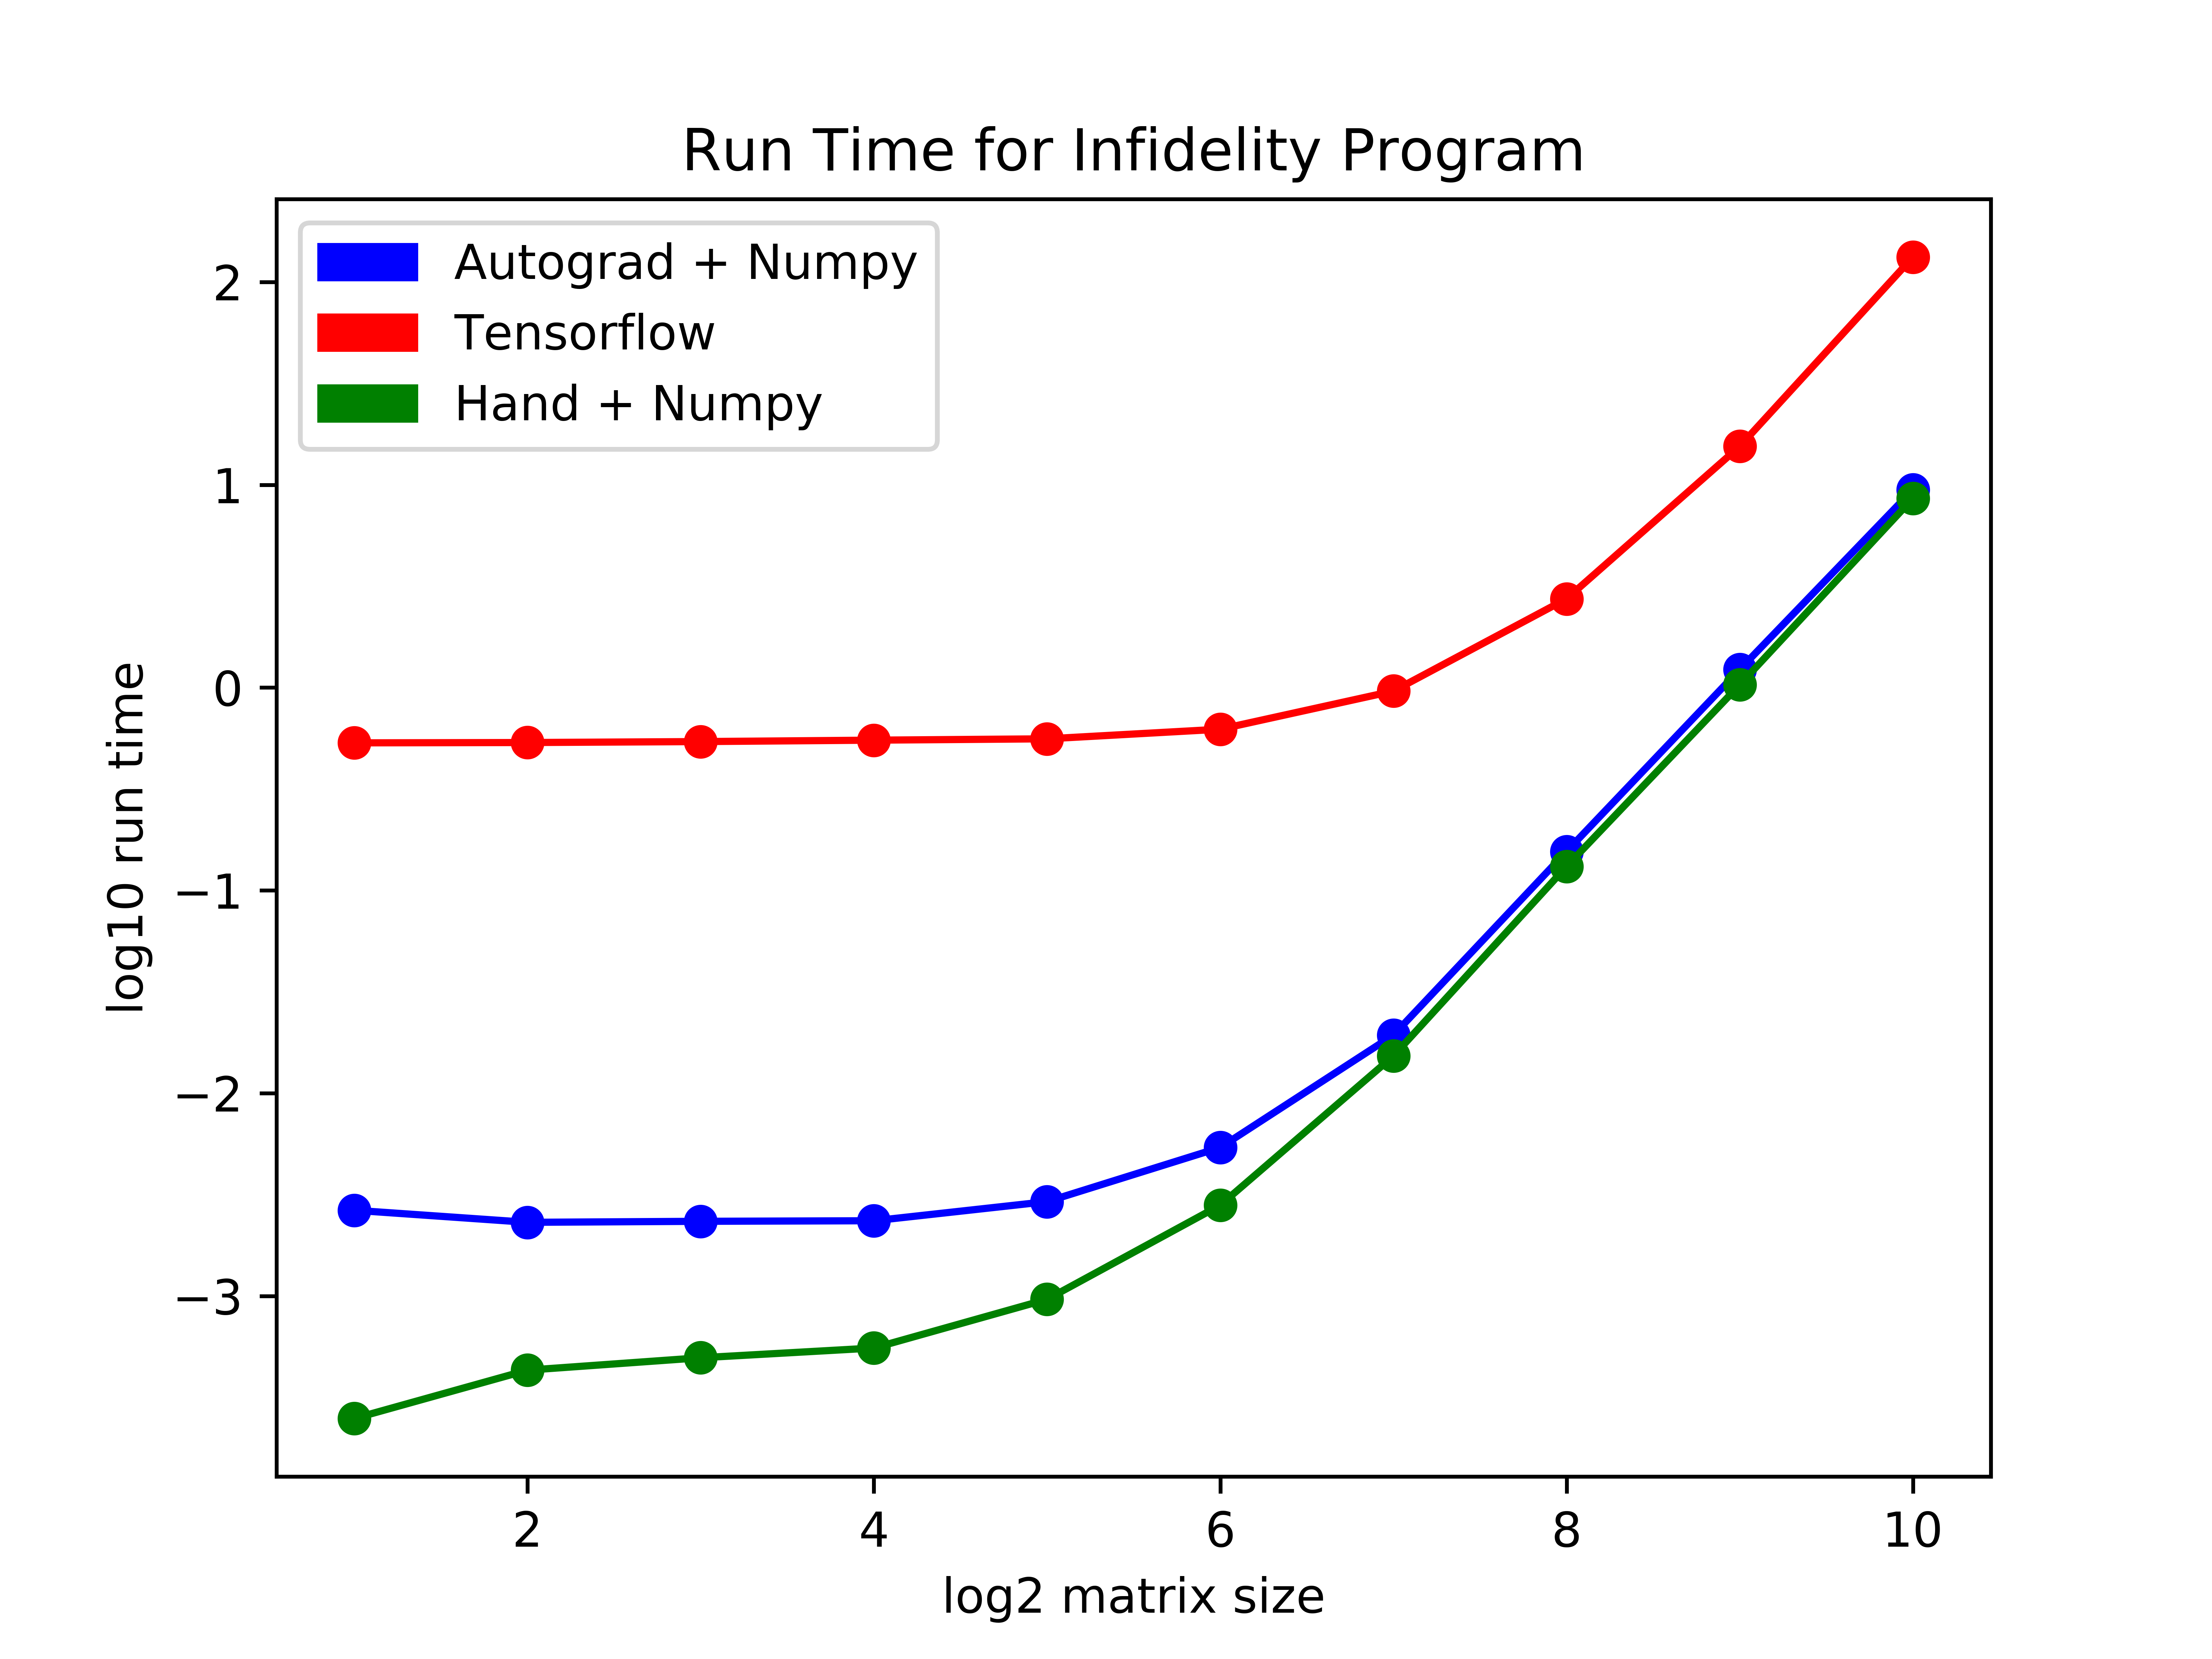
\includegraphics[width=\linewidth]{data/run_time_test.png}
  \caption{Plots corresponding to the data in Table 1.}
\end{figure}

\begin{figure}
  %% 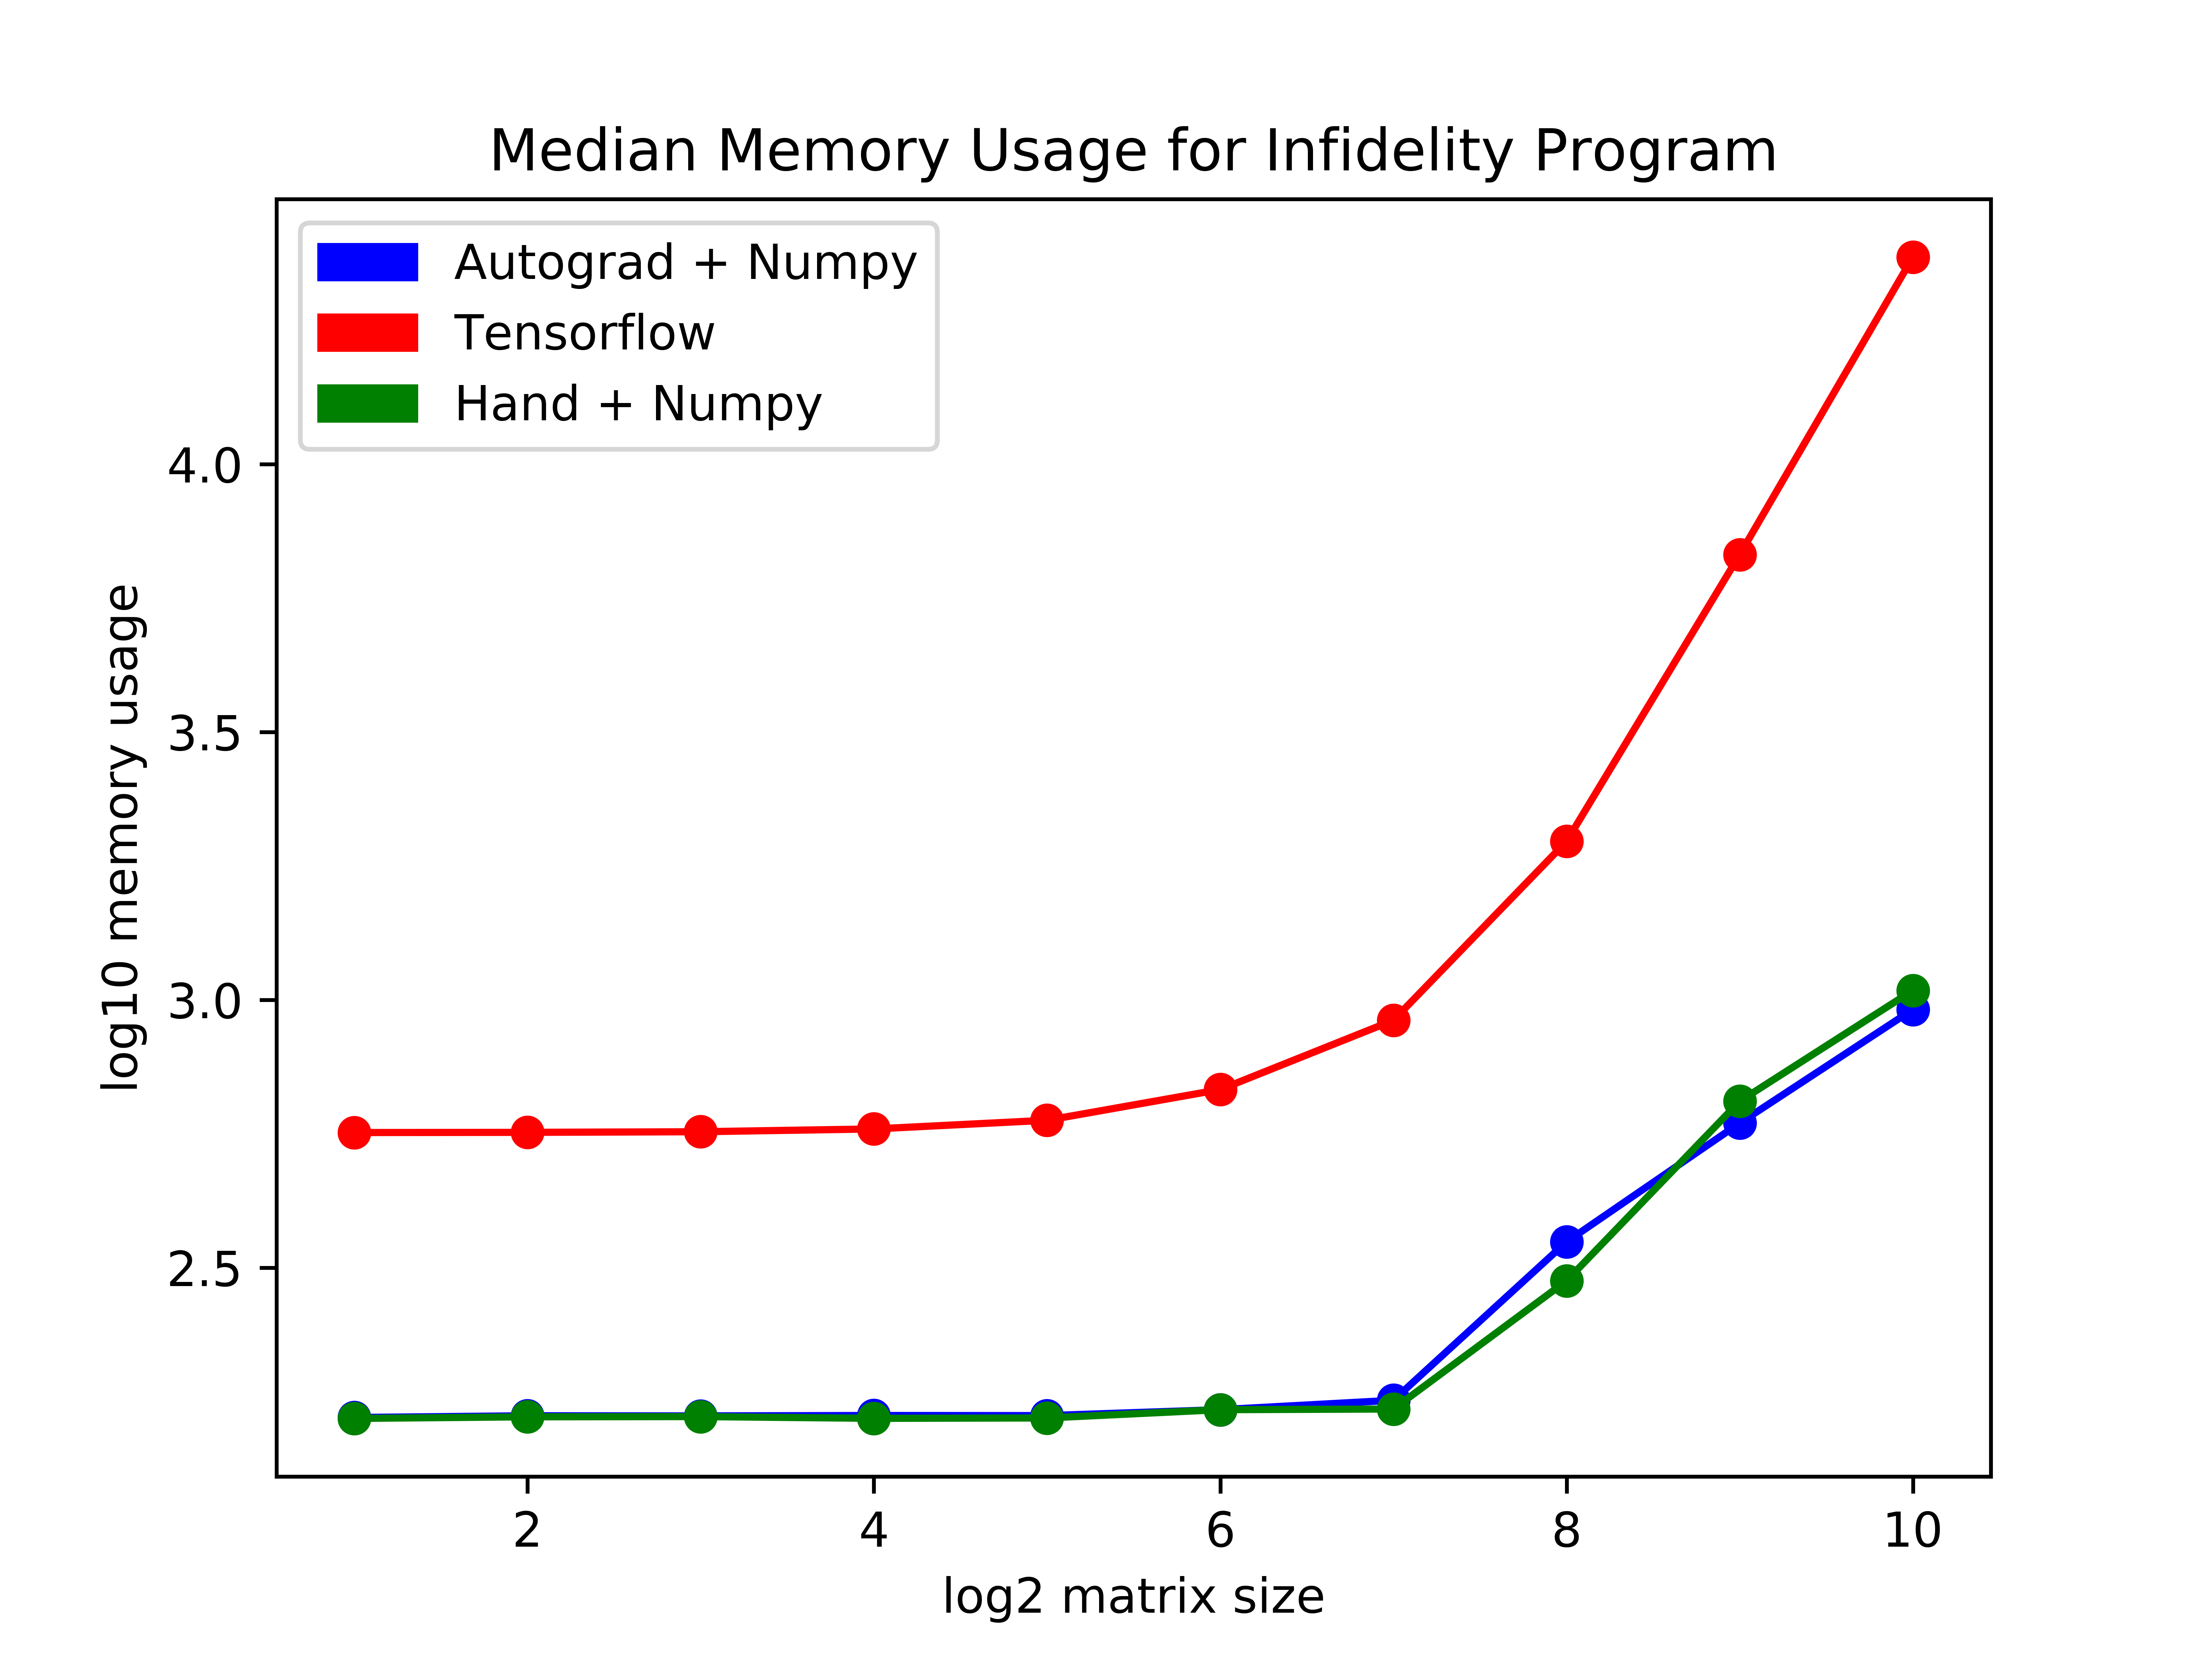
\includegraphics[width=\linewidth]{data/memory_usage_test.png}
  \caption{Plots corresponding to the data in Table 2.}
\end{figure}



\begin{table}
  \begin{center}
    \begin{tabular}{c | c | c | c}
      Time Step Count & Autograd + Numpy & Hand Derivative + Numpy\\
                      & (s)              & (s)\\
      \hline
      $10^{0}$        &  0.00669          &  0.00965\\
      $10^{1}$        &  0.06077          &  0.05672\\
      $10^{2}$        &  0.56588          &  0.44039\\
      $10^{3}$        &  5.33935          &  4.25835\\
      $10^{4}$        & 55.45920          & 43.60220\\
    \end{tabular}
  \end{center}
  \caption{Backpropagation times in seconds for the infidelity program with multiple time steps. A random initial state, target state, drift hamiltonian, control hamiltonians, and control amplitudes were generated. The control amplitudes were dotted with the control hamiltonians, which were added to the drift hamiltonian and exponentiated to get a unitary transformation. The unitary transformation was then applied to the initial state to get a final state. The infedlity (1 - $|<>|$) of the target state and final state was computed. The backward derivative of the infidelity with respect to the control amplitudes was calculated. The hand derivative method took advantage of the fact that the state was propagated by unitary transformations. The size of the hilbert space was chosen to be $2^{6}$ based on the results in Table 1 and Table 2 to garauntee fixed overhead was avoided. 10 control hamiltonians and amplitudes were used at each time step. Results reported are the mean over 10 trials. Computations were run on Fermium with 1 CPU. Fermium has an Intel i7-6700k @ 4.00GHz chip.}
\end{table}

\begin{table}
  \begin{center}
    \begin{tabular}{c | c | c | c}
      Time Step Count & Autograd + Numpy & Hand Derivative + Numpy\\
                      & (MB)             & (MB)\\
      \hline
      $10^{0}$        & 165.40039        & 162.91992\\
      $10^{1}$        & 203.94922        & 188.88867\\
      $10^{2}$        & 284.78906        & 267.52734\\
      $10^{3}$        & 515.20703        & 267.42188\\
      $10^{4}$        & 2759.4727        & 271.37109\\
    \end{tabular}
  \end{center}
  \caption{Backpropagation median memory usage over program lifetime in megabytes for the infidelity computations with multiple time steps (see Table 3). Memory usage was sampled every 0.1s. The trials here and in Table 3 were performed seperately. Results reported are the median memory usage for a program running 10 trials. Computations were run on Fermium with 1 CPU. Fermium has an Intel i7-6700k @ 4.00GHz chip.}
\end{table}

\begin{figure}
  %% 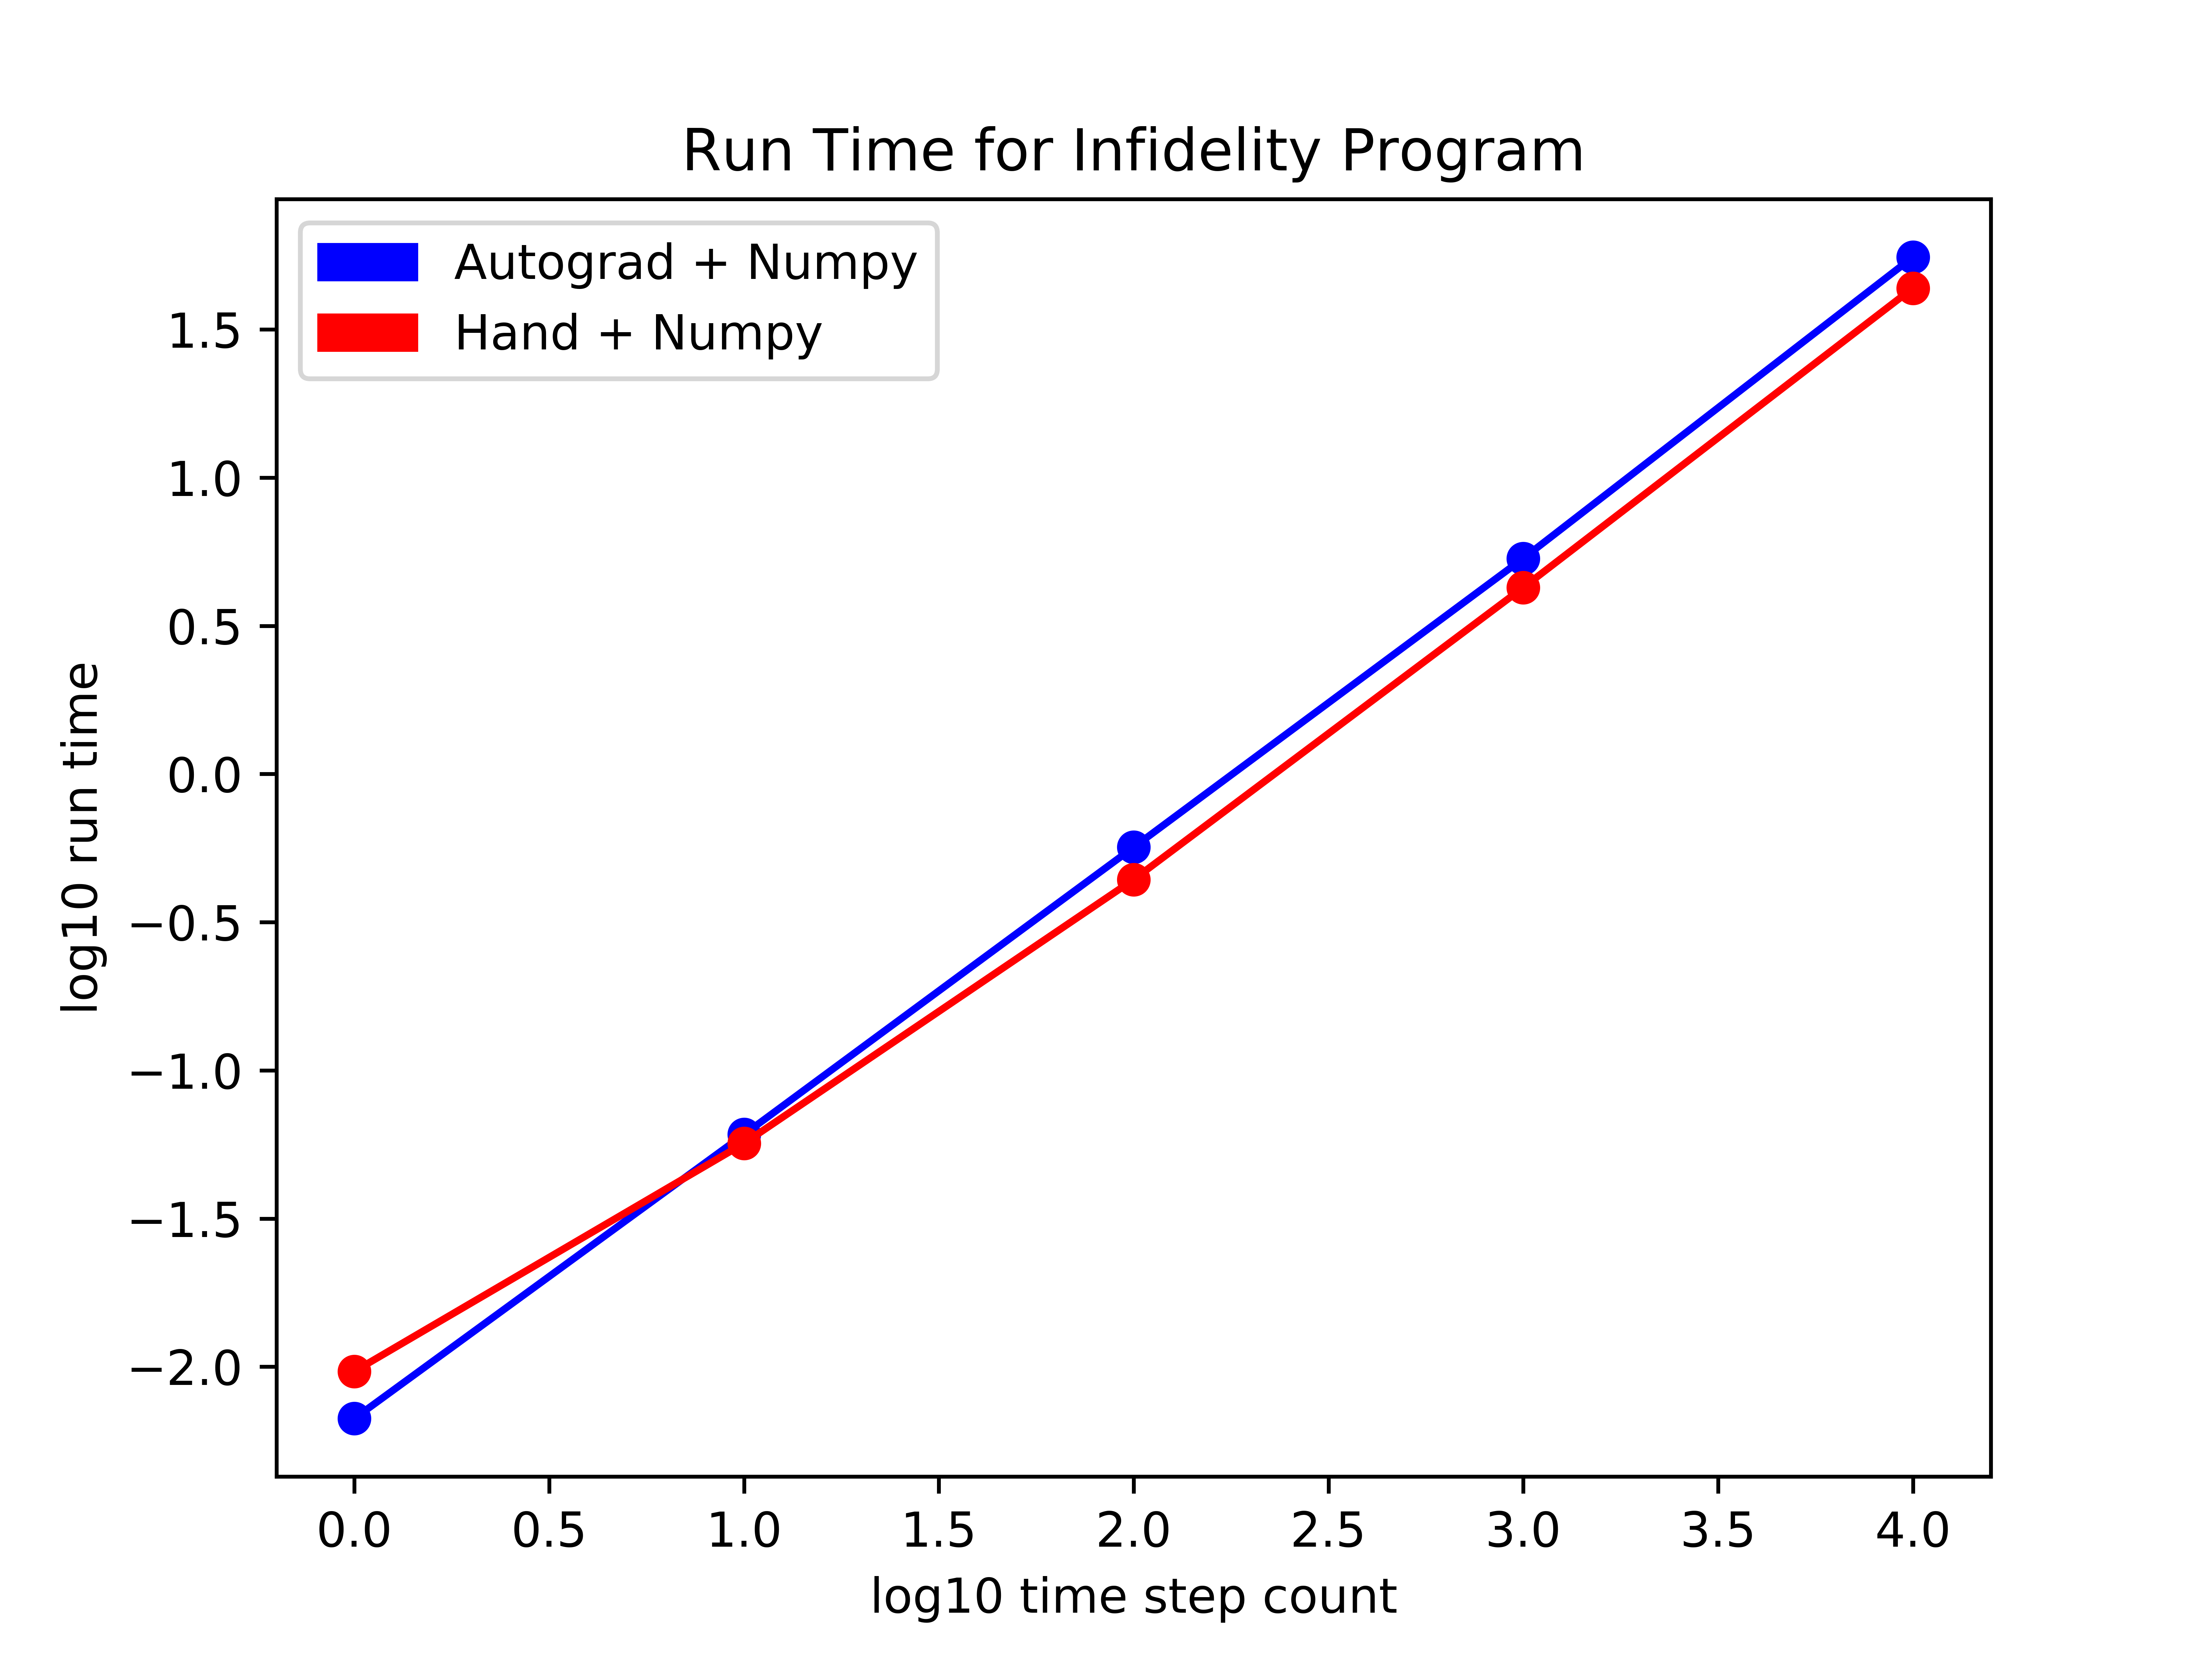
\includegraphics[width=\linewidth]{data/bpt2_run_time_plot.png}
  \caption{Plots corresponding to the data in Table 3.}
\end{figure}

\begin{figure}
  %% 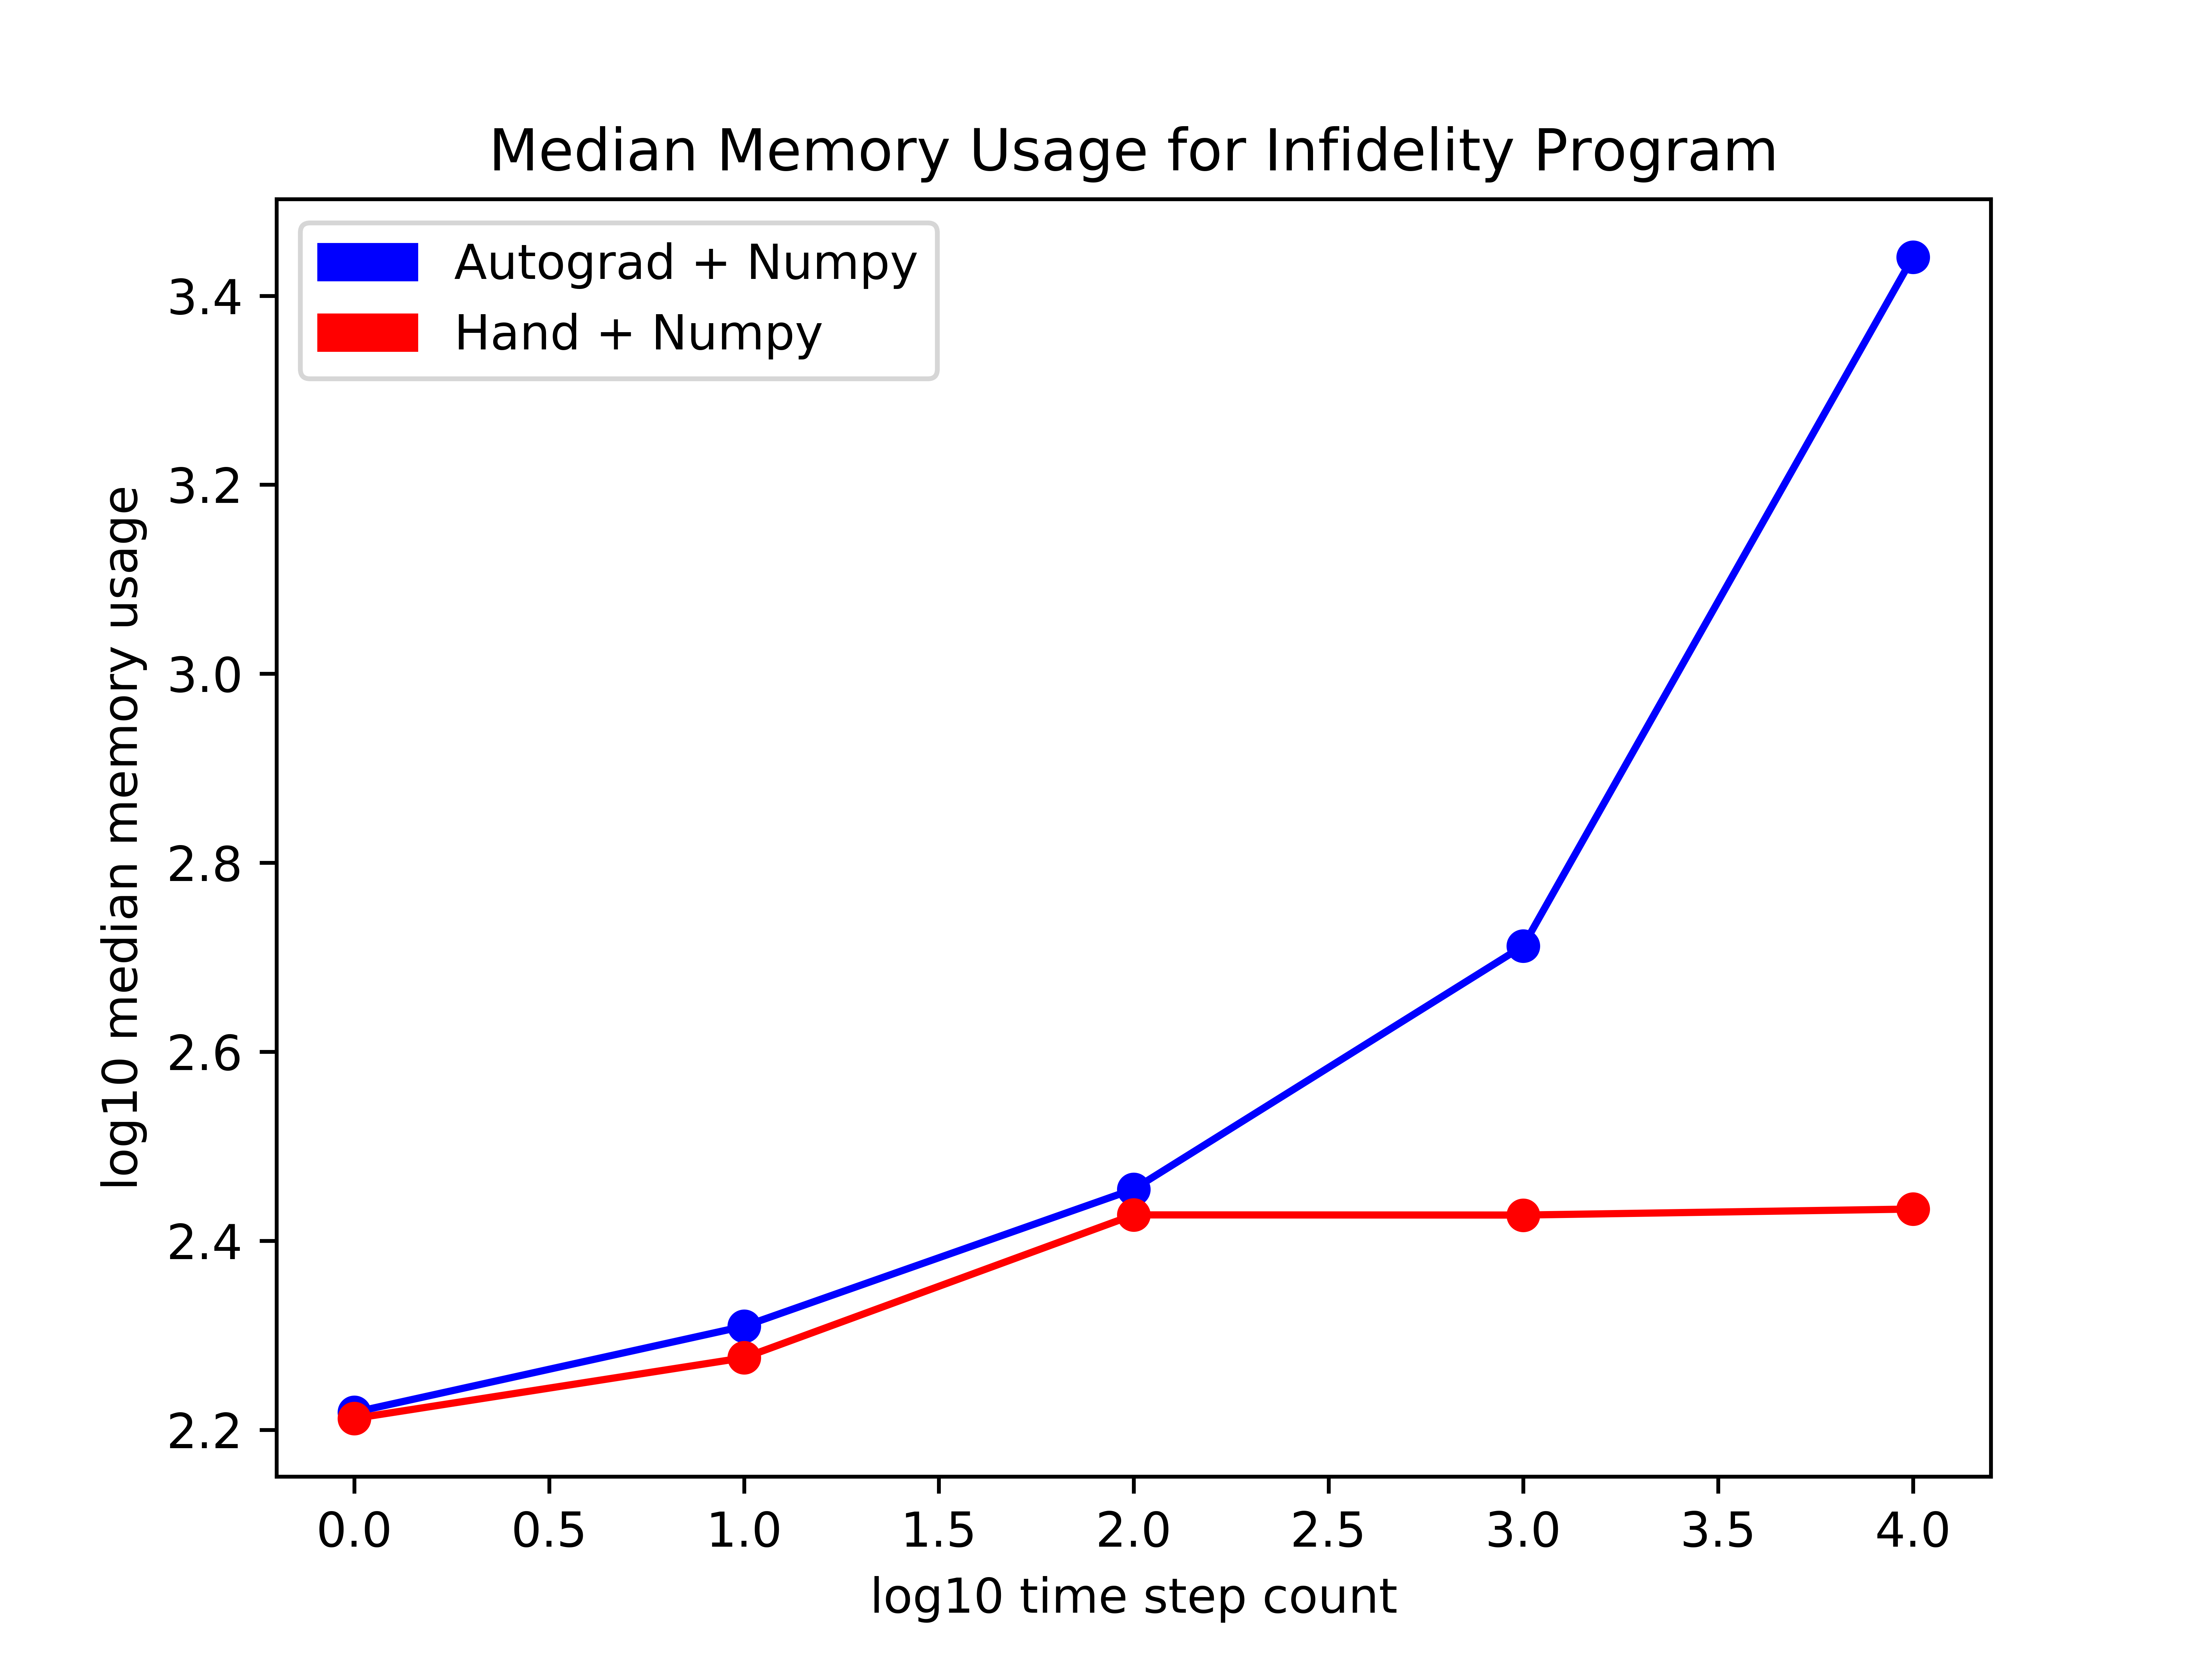
\includegraphics[width=\linewidth]{data/bpt2_memory_plot.png}
  \caption{Plots corresponding to the data in Table 4.}
\end{figure}

\section{Hamiltonian Specification}
The total hamiltonian (drift hamiltonian plus control hamiltonians) at each time step will be specified by providing a function to GRAPE that returns a hamiltonian $H_{j}$given the control operators for a time step $\{u_{j}\}$ and an integer $current\_step \in \{0, ..., steps - 1\}$. This will allow the user to perform arbitrary operations between $\{u_{j}\}$ and the control hamiltonians. This will allow the user to use time-dependent drift and control hamiltonians. The user could draw hamiltonians from a list indexed by the optimization step $current\_step$. This requires storing $steps$ number of matrices in memory and is not advised. Additionally, the user could get the wall time of the optimization by computing $t = current\_step * step\_count / pulse\_time$ to use accordingly. Autograd will allow us to get the gradient of this user-specified function with respect to $\{u_{j}\}$ for each time step.

All problems in GRAPE 2.0 will be framed as state (column vector) transfer problems. A set of initial states, and final states they map to, will be specified. Transferring an entire unitary is equivalent to transferring all basis states of the hilbert space.

\section{Cost Functions}
Cost functions will subclass a super cost function class. Each function will be instantiated with a corresponding weight and constants it requires. For example, the forbidden state cost function would be instantiated with a list of states that it is forbidding. The class will implement a method that computes a cost. The output of all cost functions should be normalized to 1. This will make it easier to choose cost function weights.

The inputs to the cost functions will be parameters of the optimization. Obviously, we must compute $\{u_{k, j}\}$ and expose them to the cost functions. Whether we provide intermediate states $\{\Psi_{j}\}$, intermediate propagators $\{U_{j}\}$, and/or total propagators $\{K_{j}\}$ is a question of memory. Suppose we have an optimization running on a hilbert space of size $2^{16}$, i.e. 16 qubits, and use 1000 optimization steps. If we use 128-bit percision complex numbers, storing $\{K_{j}\}$, $\{U_{j}\}$, and $\{\Psi_{j}\}$ together would require $128 * (2 * (2 ^{16})^{2} + 2^{16}) * 1000$bits $= 137.4$ terabytes.

Conversely, we could compute each $U_{j}$, use it to propagate the most recent $K_{j-1}, \Psi_{j-1} \rightarrow K_{j}, \Psi{j}$ and then discard $U_{j}$. We could then give $K_{j}$ and $\Psi_{j}$ to the cost function at each iteration, compute the cost and gradients for that time step and store them. This would only be required for cost functions that need to be computed for each time step, e.g. forbidden states. Functions such as target fidelity need only be evaluated at the end of optimization. The cost of a function call at each time step will add computational latency. However, only keeping, at most, $U_{j}, K_{j}, \Psi_{j}$ in memory at the same time would result in massive savings for large step sizes at large hilbert space dimensions. This would reduce memory usage in the above example from 137.4 terabytes to .1374 terabytes--a reduction that scales with the number of steps $10^{3}$.

Furthermore, we could discard propagating $K_{j}$ for state transfer problems and $\Psi_{j}$ for gate problems. In light of this analysis, each cost function class will specify if it needs to be called at each iteration, if it needs access to $\Psi_{j}$, and if it needs access to $K_{j}$. The optimization can then avoid using unecessary memory and time accordingly.

Dave believes that we should disregard $K_{j}$ altogether. Instead, he would have each problem specified as a state transfer or multi-state transfer problem. Note that a unitary transfer problem is the same as a multi-state transfer problem on the basis states. It may be more efficient to propagate a matrix in the case of the multi-state transfer; I suspect that performing $n$ matrix-vector multiplications is slower than performing one matrix-matrix multiplication where the second matrix has $n$ columns. If matrices are stored in row-major order, however, the matrix-matrix multiplication may be slower because the values ofeach column are spaced further apart in memory.

Computing gradients at each time step and adding them to a total gradient sum means that we cannot have cost functions that compute non-linear combinations of the costs they achieve at each time step. E.g. costs computed at different time steps can only be summed. Otherwise, it would be difficult to compute the gradient of that non-linear cost contribution to the total cost function. However, we don't anticipate needing this functionality.

\section{Numerical Compuatation Performance}
GRAPE 2.0 will expose more sophisticated methods for calculating the time-dependent schroedinger equation propagator. Namely, it will implement the second, fourth, and sixth order mangus integrator methods with commutators described in \cite{auer2018magnus}. More details can be found in \cite{blanes2009magnus}. I will try implementing the mutliple-exponential magnus integrators described in \cite{auer2018magnus} and compare their run time to the commutator methods. However, I expect that the commutator methods will be faster because I expect matrix exponentiation to be more expensive than matrix multiplication (see Table 5). Note that GRAPE 1.0 uses the second order magnus integrator method $U = \textrm{exp}(-i H \delta t)$.

GRAPE 2.0 could calculate the matrix exponential and the derivative of the matrix exponential using \href{https://docs.scipy.org/doc/scipy-0.14.0/reference/generated/scipy.linalg.expm_frechet.html}{scipy.linalg.expm\_frechet}. Scipy's algorithm \href{https://docs.scipy.org/doc/scipy-0.14.0/reference/generated/scipy.linalg.expm.html#scipy.linalg.expm}{scipy.linalg.expm} takes longer to perform than the algorithm used in GRAPE 1.0 for the $T = 10$ case (see Table 5 and Figure 9). However, Scipy's algorithm is more numerically accurate because it accounts for floating point round-off error \cite{al2009new}.

Note that if the drift and control hamiltonians are hermitian, then their linear combination with real coefficients is hermitian. Therefore, the system hamiltonian may be \href{https://en.wikipedia.org/wiki/Matrix_exponential#Computing_the_matrix_exponential}{diagonalized and exponentiated} easily. Similarly, the derivative of the matrix exponential for a diagonal matrix $A$ is given by $\frac{\partial}{\partial t} e^{A(t)} = e^{A(t)} \frac{\partial A(t)}{\partial t}$ which is easy to compute given the original exponentiated matrix. In particular, the matrix we exponentiate will be skew hermitian since $U = exp^{-i H \delta t}$ with $H$ hermitian. Since skew hermitian matrices are diagonalizable, we may consider an efficient matrix exponentiation algorithm with diagonalization.
\begin{table}
  \begin{center}
    \begin{tabular}{c | c | c | c}
      Matrix Size & Scipy & GRAPE 1.0, T = 10 & GRAPE 1.0, T = 20\\
      \hline
      $2^{1}$  & 0.000237 & 0.000057 & 0.000091\\
      $2^{2}$  & 0.000184 & 0.000058 & 0.000094\\
      $2^{3}$  & 0.000206 & 0.000062 & 0.000100\\
      $2^{4}$  & 0.000227 & 0.000079 & 0.000125\\
      $2^{5}$  & 0.000334 & 0.000134 & 0.000203\\
      $2^{6}$  & 0.001352 & 0.000353 & 0.000488\\
      $2^{7}$  & 0.002921 & 0.001032 & 0.001622\\
      $2^{8}$  & 0.016121 & 0.003776 & 0.006518\\
      $2^{9}$  & 0.047553 & 0.029418 & 0.049804\\
      $2^{10}$ & 0.274228 & 0.250185 & 0.418202\\
      $2^{11}$ & 2.121346 & 1.965816 & 3.065884\\
    \end{tabular}
  \end{center}
  \caption{Matrix exponentiation run times in seconds for Scipy and GRAPE 1.0 respectively. The reported values are the average over 100 matrices. All matrices are dense square matrices with row and column lengths equal to the reported matrix size. For GRAPE 1.0, the scaling factor $p$ is chosen such that $\frac{||A||}{2^{p}} \le 1$. $T$ corresponds to the number of taylor terms chosen for the GRAPE 1.0 algorithm. Computations were run on Fermium. Fermium has an Intel i7-6700k @ 4.00GHz w/ 8 CPUs.}
\end{table}

\begin{figure}
  %% 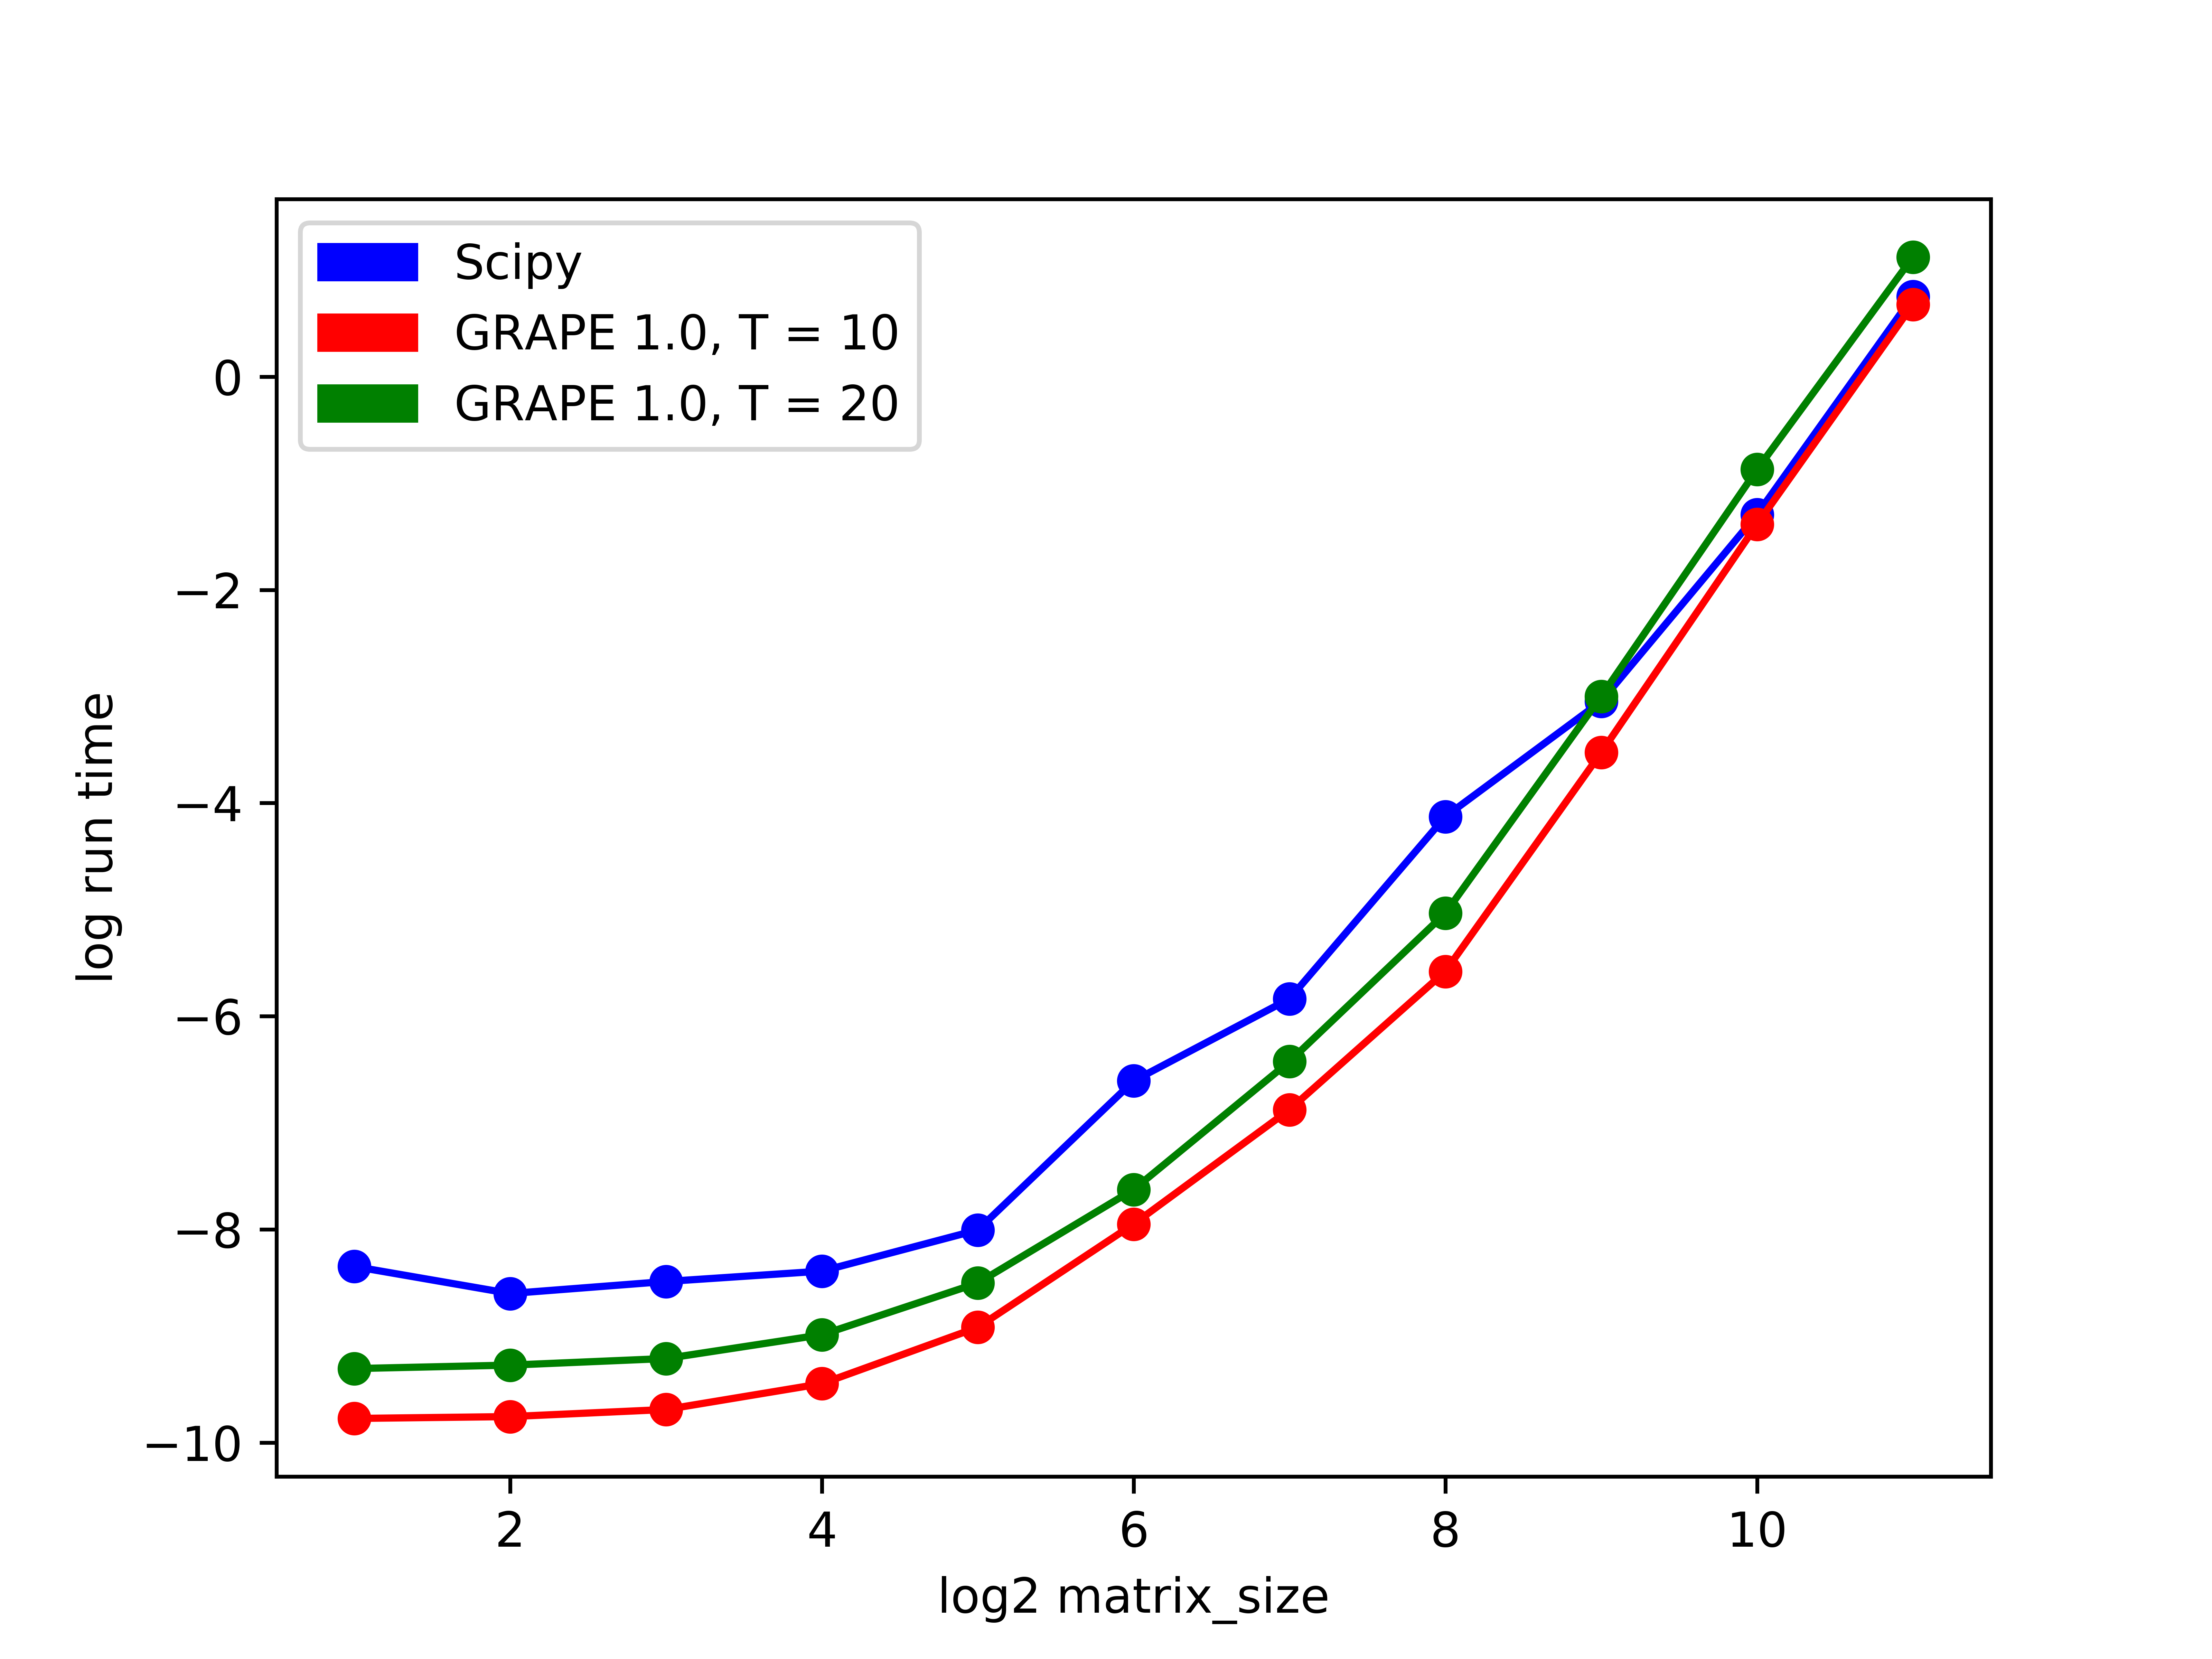
\includegraphics[width=\linewidth]{data/expm.png}
  \caption{Plot corresponding to the data in Table 5.}
\end{figure}

\section{Time Discretization}
Sometimes we have a parameter in our system Hamiltonian that acts very quickly. Consider $H = \omega_{c}a^{\dagger}a$ where $\omega_{c} = 5$GHz. The osciallation of our system is on the order of $\frac{1}{5\textrm{GHz}} = \frac{1}{5}$nanoseconds. This suggests that we use an evolution time step of $\frac{1}{5}$ns. However, the sampling rate of our arbitrary waveform generator may only be 1 sample per ns. We typically get around this problem by performing a rotating frame transformation to our system Hamiltonian (e.g. $U=\textrm{exp}(i\omega_{c}a^{\dagger}at)$) that cancels the term $\omega_{c}a^{\dagger}a$ in our Hamiltonian. Consider a case where no such simple rotating frame transformation exists or where it makes the other terms in the Hamiltonian prohibitively hard to compute. In GRAPE 1.0 we cannot differentiate between the system rate and the sampling rate, so we must optimize the control pulse at $\frac{1}{5}$ steps per nanosecond even though we cannot realize the output pulse. In GRAPE 2.0 we could implement a scheme where control amplitudes are updated at one time step, but the system evolves at another. Let the rate at which we update the discrete pulse be known as the pulse rate. Let the rate at which we must account for changes in our system be known as the system rate. The optimization parameters will be updated at pulse steps and interpolated at system steps. The user will provide an interpolation scheme which will be differentiated with autograd. The gradient of each of the parameters will be calculated at both pulse and system steps. For simplicity, the number of system steps must be an integer multiple of the pulse steps.

Another way to overcome this obstacle is to optimize an analytical pulse to fit the specified problem. The optimization problem then turns to optimizing the parameters of the anlaytical pulse. Note that these optimization parameters act on the system for all time steps, as opposed to the discrete case. Since the pulse is continuous in time, its value does not need to be interpolated numerically. Therefore, there is no need to differentiate between a system and pulse time step for this case. GRAPE 2.0 will implement both a discrete and a continuous strategy seperately.

\section{Open System}
If our system can be modeled as an open markovian system, we may account for dissipative processes by evolving the probability density matrix $\rho$ under the \href{https://en.wikipedia.org/wiki/Lindbladian}{Lindbladian}
\[
\dot{\rho} = -i[H, \rho] + \Gamma(p) = \mathcal{L}(p)\textrm{.}
\]
Note that if $\Gamma(p) = 0$ for all time then the Lindbladian reduces to the Schroedinger equation, the PDE we ordinarily evolve under.

Implementing this evolution is computationally analogous to implementing the evolution of a unitary $U$ under the Schroedinger equation. Thus, to implement this evolution, we can use the same methods as discussed above. We need to propagate $\rho$ through a series of transformations at time step j of $L_{j} = exp(\mathcal{L}_{j}\delta t)$. Note that methods have been developed to simulate Lindbladian evolution without matrix exponentiation \cite{cleve2016efficient}. However, these methods incur some error, do not garauntee proper treatment of floating point arithmetic out of the box, and are not garaunteed to give a speedup over matrix exponentiation for our use case. For example, the cited method requires representation of the Lindbladian as a string of kronecker products of pauli matrices. I find it hard to believe performing a decomposition of this type would be time efficient given the matrix exponentiation times reported above (Table 5).

The cost functions for this evolution method will be dependent upon the probability density matrix at some time step, rather than states or unitaries. I expect the most useful cost function to be $C \propto -|Tr(\rho^{\dagger}_{T} \rho_{N})|$ to maximize the realization of a target probability density matrix.

In this case, we evolve probability density matrices under the PDE instead of individual state vectors. Thus, for each state we wish to transform, we will need to specify a corresponding probability density matrix \cite{basilewitsch2019reservoir}. Similar to the Schroedinger equation case, the function to evolve under the Lindbladian will require a set of initial probability density matrices and corresponding final probability density matrices. The reader should see why this is more expensive than our previous task. If we want to evolve every basis state in the hilbert space, instead of requiring the evolution of $d$ vectors of length $d$, we must now evolve $d$ matrices of size $d \times d$. Note that we expect the probability denisty matrices to be sparse, so we should see reasonable speedups by employing sparse multiplication. We may also employ the technique of turning each probability density matrix to a column vector of length $d^{2}$ and the Lindbladian superoperators to matrices of size $d^{2} \times d^{2}$. I will run tests to see which of these options is most memory and time efficient. If the matrices are stored in row-major order, then the memory layout of the probability density matrix should be the same in matrix and column vector format, so I wouldn't expect better cache performance. Further, increasing the size of the Lindbladian superoperators would seem to give worse cache performance because redundant values need to be referenced from different locations in memory.

\section{Further Performance Considerations}
Autograd implements gradients for numpy operations. Numpy operations are currently limited to running on CPUs, although it takes advantage of access to multiple CPUs for parallelism. Furthermore, Scipy's sparse matrix operations are not currently supported by autograd. To overcome this obstruction, we could implement derivates for these functions by hand or extend autograd.

GRAPE 2.0 will use \href{https://scikit-cuda.readthedocs.io/en/latest/}{scikit-cuda} on top of \href{https://documen.tician.de/pycuda/}{PyCUDA} to perform GPU operations. GRAPE 2.0 will extend autograd to provide derivatives of scikit-cuda functions. Sparse matrix operations are implemented by \href{https://pyculib.readthedocs.io/en/latest/cusparse.html}{cuSPARSE}.

\section{Gradient Based Optimization}
The question is: Which gradient-based optimizer should we use? GRAPE 1.0 made use of Adam and L-BFGS-B. GRAPE 2.0 will allow the user to create their own optimizer classes to provide updates to learning parameters. GRAPE 2.0 will implement Adam, Adadelta, and L-BFGS-B natively. Adam and Adadelta will be implemented following their \href{https://github.com/keras-team/keras/blob/master/keras/optimizers.py}{keras implementations}. L-BFGS-B will use the \href{https://docs.scipy.org/doc/scipy/reference/optimize.minimize-lbfgsb.html}{scipy implementation}. Adam and L-BFGS-B were chosen because they yielded good results in GRAPE 1.0. Adadelta was chosen because it requires less memory than Adam. Adam needs to store information about all of the parameters it is optimizing. This memory usage scales poorly for $10,000 <$ learning parameters. If time allows, both Dave and I think it would be interesting to see if providing hessians to L-BFGS-B would be useful. I also think it would be interesting to try Newton's method if we have access to hessians. Second-order methods should be more expensive, but I think if they yield better performance they would be worth the value. We care about achieving a specific tolerance for our cost functions, e.g. time, fidelity, etc. The main constraint in constructing higher order derivatives is that we need to be able to take higher order derivatives of the matrix exponential, which likely means implementing a custom solution. I may be thinking about this the wrong way and there is an easier approach.

\section{Software Design}
GRAPE 2.0 will be python3 official and linted. It will adhere to \href{https://www.python.org/dev/peps/pep-0008/}{PEP8}. It will have unit tests on its modules.

\section{Miscellaneous Features}
\begin{enumerate}
\item Examples to include: Gate Smash, HPO.
\item Include a library of hamiltonians.
\end{enumerate}


\bibliography{report/refs}
\bibliographystyle{plainnat}

\end{document}
